\documentclass[tikz,border=4pt]{standalone}
% Estilo común de los diagramas de bloques (se usa con \input en cada standalone)
\usepackage[defaultsans,scale=0.92]{lato}
\usepackage{libertinust1math}
\usepackage{xcolor,amsmath}
\usepackage{tikz}
\usetikzlibrary{positioning,arrows.meta,calc,shapes.geometric}
\usepackage{../../notacion}
\definecolor{ctrlazul}{HTML}{1E5AA8}\definecolor{ctrlnoche}{HTML}{14213D}
\definecolor{ctrlcoral}{HTML}{D1495B}\definecolor{ctrlverde}{HTML}{2A9D8F}
\definecolor{ctrlambar}{HTML}{E09F3E}\definecolor{ctrlgris}{HTML}{5C677D}
\definecolor{ctrlvioleta}{HTML}{6C4AB6}\definecolor{ctrlteal}{HTML}{0F7173}
\tikzset{
  >={Stealth[length=2.4mm]}, every node/.style={font=\small},
  bloque/.style={draw=ctrlnoche,fill=ctrlazul!7,thick,rounded corners=1.5pt,minimum height=9mm,minimum width=13mm,inner sep=4pt},
  suma/.style={draw=ctrlnoche,thick,circle,inner sep=0pt,minimum size=6mm},
  senal/.style={->,thick,draw=ctrlnoche},
  rot/.style={font=\footnotesize,text=ctrlgris},
}

\begin{document}
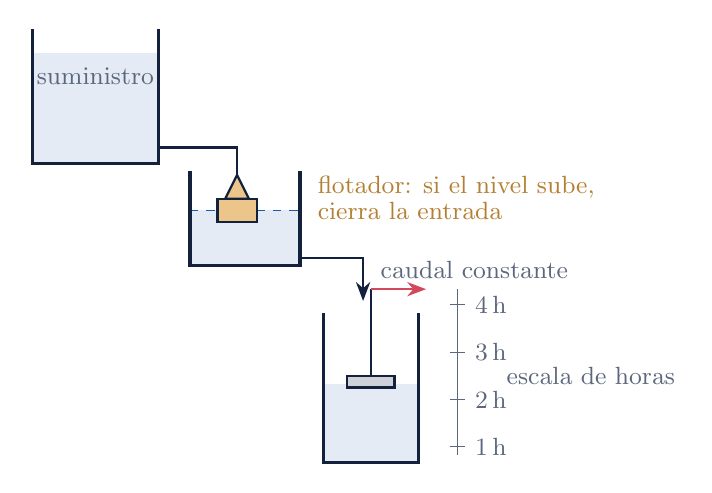
\begin{tikzpicture}[font=\footnotesize]
  % depósito de suministro
  \fill[ctrlazul!12] (0,2.2) rectangle (1.6,3.6); \draw[very thick,ctrlnoche] (0,3.9)--(0,2.2)--(1.6,2.2)--(1.6,3.9);
  \node[ctrlgris] at (0.8,3.3) {suministro};
  \draw[thick,ctrlnoche] (1.6,2.4)--(2.6,2.4)--(2.6,2.05);
  % recipiente regulador
  \fill[ctrlazul!12] (2.0,0.9) rectangle (3.4,1.6); \draw[ctrlazul,dashed] (2.0,1.6)--(3.4,1.6);
  \draw[very thick,ctrlnoche] (2.0,2.1)--(2.0,0.9)--(3.4,0.9)--(3.4,2.1);
  % flotador cónico
  \draw[thick,ctrlnoche,fill=ctrlambar!60] (2.35,1.45) rectangle (2.85,1.75);
  \draw[thick,ctrlnoche,fill=ctrlambar!60] (2.45,1.75)--(2.75,1.75)--(2.6,2.05)--cycle;
  \node[ctrlambar!80!black,anchor=west] at (3.5,1.9) {flotador: si el nivel sube,};
  \node[ctrlambar!80!black,anchor=west] at (3.5,1.6) {cierra la entrada};
  % salida constante
  \draw[thick,ctrlnoche] (3.4,1.0)--(4.2,1.0)--(4.2,0.6); \draw[senal] (4.2,0.75)--(4.2,0.45);
  \node[anchor=west,ctrlgris] at (4.3,0.85) {caudal constante};
  % recipiente receptor
  \fill[ctrlazul!12] (3.7,-1.6) rectangle (4.9,-0.6); \draw[very thick,ctrlnoche] (3.7,0.3)--(3.7,-1.6)--(4.9,-1.6)--(4.9,0.3);
  \draw[thick,ctrlnoche,fill=ctrlgris!30] (4.0,-0.65) rectangle (4.6,-0.5);
  \draw[thick,ctrlnoche] (4.3,-0.5)--(4.3,0.6); \draw[thick,ctrlcoral,->] (4.3,0.6)--(5.0,0.6);
  \foreach \y/\h in {-1.4/1,-0.8/2,-0.2/3,0.4/4} {\draw[ctrlgris] (5.3,\y)--(5.5,\y) node[right]{\h\,h};}
  \draw[ctrlgris] (5.4,-1.5)--(5.4,0.6);
  \node[anchor=west,ctrlgris] at (5.9,-0.5) {escala de horas};
\end{tikzpicture}
\end{document}
